
\chapter{Theoretical Background and Related Work}
\label{chap:background}

\section{Domain and Subdomain of the Thesis}

The thesis belongs to the broad domain of artificial intelligence applied to computational neuroscience. More specifically, it is situated at the intersection of brain decoding, representation learning, and generative modelling. The subdomain addressed here is \emph{visual perception decoding from fMRI}: given a measured cortical response, the goal is to recover information about the external image stimulus that produced it. This task differs from classical neuroimaging analysis because it is not limited to identifying which brain regions are active; instead, it seeks to infer \emph{what was seen} by mapping neural activity into a meaningful computational representation \cite{Kay2008,Naselaris2009}.

\section{Historical Evolution of Visual Decoding}

Visual decoding from fMRI has progressed from low-level stimulus recovery to semantically rich latent reconstruction. Early work showed that activation patterns in the visual cortex carry enough information to infer image structure and to identify natural images and naturalistic scenes \cite{Thirion2006,Kay2008,Naselaris2009,Nishimoto2011}. Subsequent work moved to deep-feature decoding and generative reconstruction with GANs and large CNN features \cite{Horikawa2017,Wen2018,Seeliger2018,Shen2019,VanRullen2019}, and the most recent phase relies on multimodal latent spaces and strong generative priors: latent-diffusion reconstructions \cite{Takagi2023,Ozcelik2023}, contrastive retrieval-plus-reconstruction frameworks (MindEye \cite{Scotti2023}), and shared-subject scaling (MindEye2 \cite{Scotti2024}). The present thesis belongs to this recent phase and emphasises retrieval-oriented latent decoding.

\section{fMRI-Based Visual Decoding}

Functional magnetic resonance imaging measures the BOLD signal, which acts as an indirect proxy for neural activity \cite{Allen2022,Wen2018}. In visual decoding tasks, the input is usually a voxel vector derived from one or more regions of interest in the visual cortex, while the target corresponds to some representation of the viewed stimulus. Earlier approaches focused on category labels or hand-crafted image descriptors \cite{Thirion2006,Kay2008,Naselaris2009}. More recent work predicts features from deep visual models, which allows the decoder to preserve semantic and structural information at a much richer level \cite{Horikawa2017,Wen2018,Scotti2023}.

Let $x_i \in \mathbb{R}^{V}$ be the voxel vector for trial $i$. A basic decoder predicts $\hat{z}_i \in \mathbb{R}^{d}$, where $z_i$ is the target visual representation extracted from the ground-truth image. Because the embedding space is usually normalized, cosine similarity becomes the natural scoring function:
\begin{equation}
\cos(\hat{z}_i, z_j) = \frac{\hat{z}_i^{\top} z_j}{\lVert \hat{z}_i \rVert_2 \, \lVert z_j \rVert_2}.
\label{eq:cosine_similarity}
\end{equation}
A retrieval system ranks all gallery items according to this similarity and checks whether the correct image is recovered near the top of the list.

\section{Natural Scenes Dataset}

The Natural Scenes Dataset is one of the most important benchmarks for high-resolution visual decoding from fMRI \cite{Allen2022}. It contains 7T fMRI responses recorded while subjects viewed thousands of natural images. The scale, signal quality, and repeated-image structure of NSD make it especially suitable for studying image-specific decoding. However, NSD also imposes strict requirements on data handling: repeated trials, image identifiers, train/validation separation, and session-level normalization must all be treated carefully to avoid leakage.

In this thesis, the practical role of NSD is twofold. First, it provides the paired $(x_i, z_i)$ examples needed for supervised learning. Second, it offers a benchmark environment in which the quality of retrieval and reconstruction can be discussed relative to recent systems such as MindEye and MindEye2 \cite{Scotti2023,Scotti2024}. The present work does not attempt to replace NSD-specific discipline with ad hoc experimentation; on the contrary, it treats split integrity and reproducibility as first-class methodological requirements.

\begin{figure}[htbp]
    \centering
    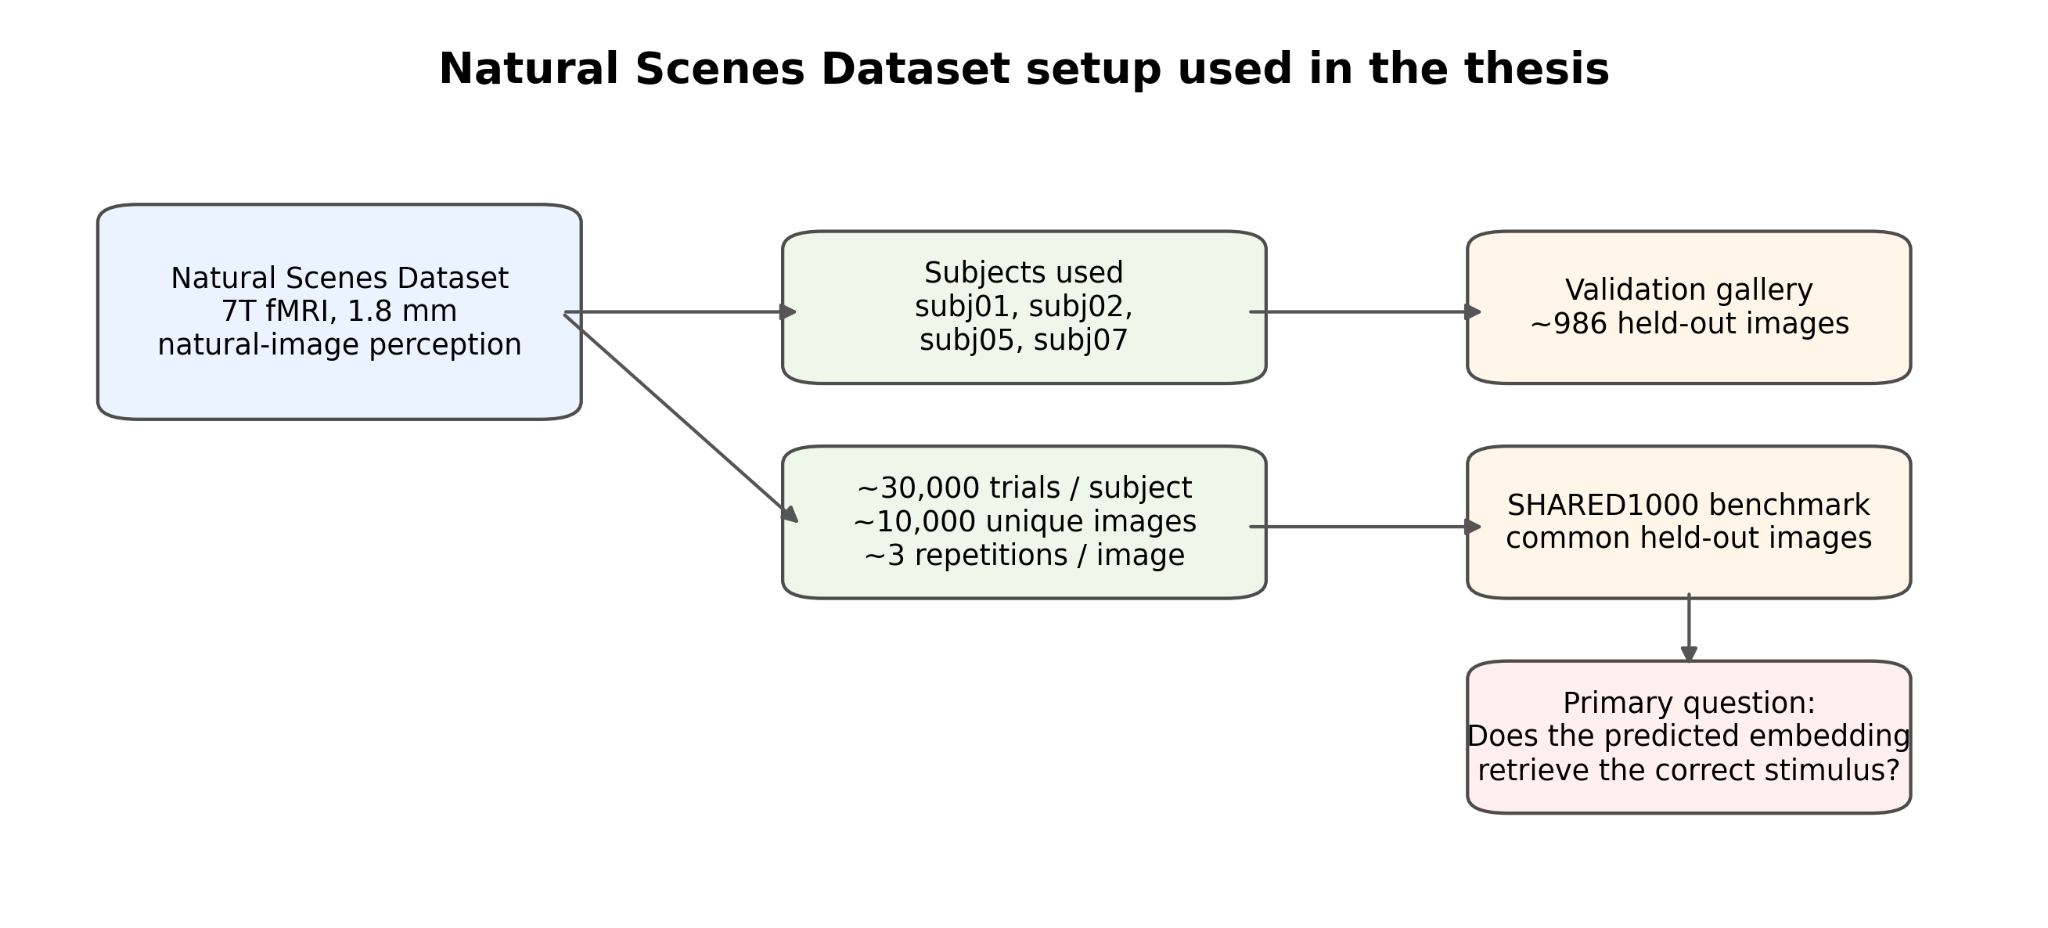
\includegraphics[width=0.96\textwidth]{nsd_overview.png}
    \caption{Dataset setting used throughout the thesis. The work is developed on the Natural Scenes Dataset under a retrieval-oriented protocol, with validation and SHARED1000 treated as the main endpoints.}
    \label{fig:nsd_overview}
\end{figure}

\section{CLIP as the Target Representation}

CLIP learns a shared representation space for images and text using large-scale contrastive supervision \cite{Radford2021}. Its image encoder produces embeddings that are semantically meaningful, well structured for nearest-neighbour search, and highly reusable across downstream tasks. For brain decoding, CLIP is useful because it provides a target space that is already organized around visual-semantic similarity.

This thesis uses CLIP-style image embeddings as latent targets instead of direct pixel supervision. The practical benefit is that the decoder does not need to reconstruct raw images directly from noisy brain signals. Instead, it predicts a representation that can support both retrieval and conditioning of a downstream generator. This idea aligns well with recent diffusion-based reconstruction pipelines \cite{Takagi2023,Ozcelik2023,Scotti2023}.

Figure~\ref{fig:clip_shared_space_alignment} illustrates the geometric intuition behind this choice. CLIP places semantically corresponding images and text descriptions in neighboring regions of a shared embedding space. In the present thesis, this shared geometry becomes the decoding target: a predicted brain embedding is useful only insofar as it lands near the correct image neighborhood while remaining separated from semantically plausible distractors.

\begin{figure}[htbp]
    \centering
    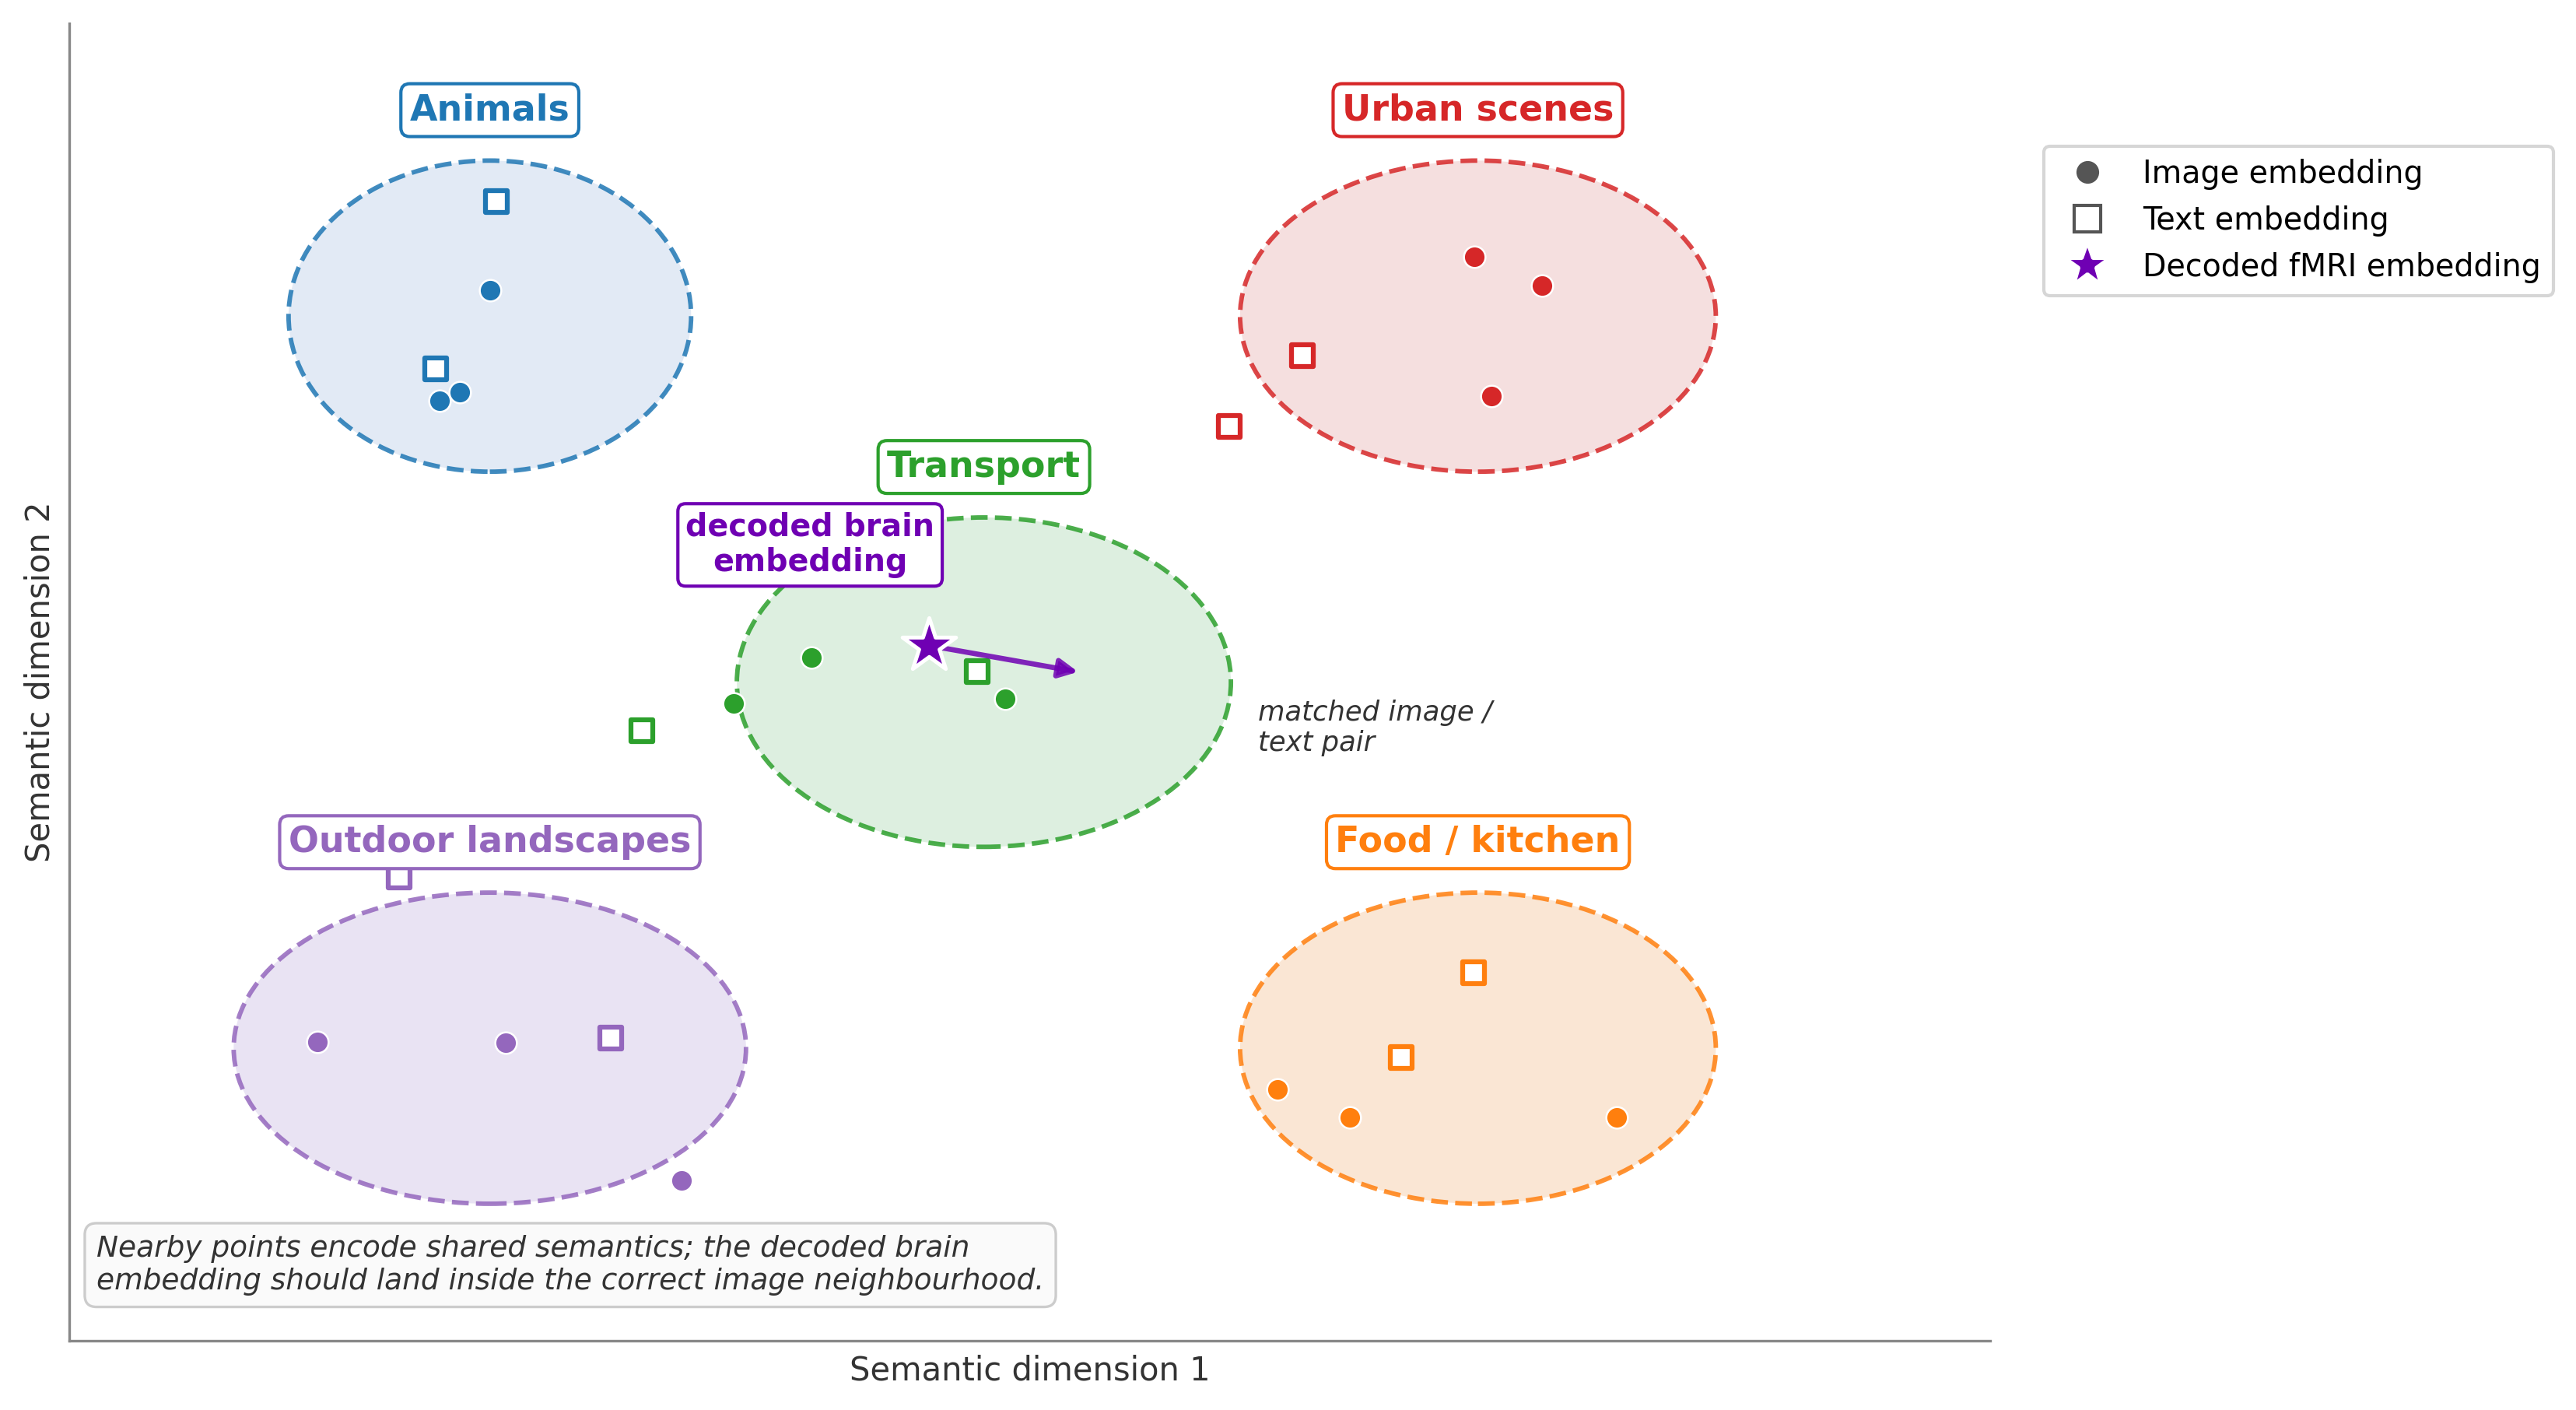
\includegraphics[width=0.96\textwidth]{clip_shared_space_alignment.png}
    \caption{Conceptual view of CLIP as a shared semantic space. Image and text embeddings for related concepts occupy nearby regions, which is why CLIP provides a meaningful target geometry for brain decoding and retrieval.}
    \label{fig:clip_shared_space_alignment}
\end{figure}

\section{Latent Diffusion Models and Generative Reconstruction}

Latent diffusion models synthesize images by iteratively denoising a latent variable conditioned on text, image, or other contextual information \cite{Rombach2022}. A forward step perturbs a clean latent $y_0$ as
\begin{equation}
y_t \sim \mathcal{N}\!\left(\sqrt{1-\beta_t}\, y_{t-1},\, \beta_t I\right),
\label{eq:diffusion_forward}
\end{equation}
and the learned reverse process recovers a clean latent conditioned on the predicted visual representation \cite{Takagi2023,Ozcelik2023}. In this thesis, reconstruction is a downstream extension; retrieval remains the main quantitative focus.

\section{Retrieval Geometry and Hubness}

Accurate latent regression is not sufficient by itself; what matters quantitatively is the geometry of the predicted embeddings relative to the gallery. High-dimensional retrieval spaces suffer from \emph{hubness}: a few gallery items become nearest neighbours for an excessive number of queries, distorting raw cosine retrieval and making a model appear less discriminative than its regression error would suggest \cite{Conneau2018}. The project therefore relies on hubness-aware scoring; the resulting distinction between latent fidelity and retrieval geometry is one of the key interpretive lessons of the experiments.

\section{Evaluation Metrics}

The core metric used throughout the thesis is Recall@K. For a predicted embedding $\hat{z}_i$ and a gallery $\mathcal{G}$, Recall@K is defined as
\begin{equation}
\mathrm{R@K} = \frac{1}{N} \sum_{i=1}^{N} \mathbf{1}\left[\operatorname{rank}(g_i^\star \mid \hat{z}_i) \leq K\right],
\label{eq:recall_at_k}
\end{equation}
where $g_i^\star$ is the ground-truth gallery image corresponding to sample $i$. In this thesis, Recall@1 is the most important endpoint because it directly measures image-specific identification.

A second important metric is cross-domain similarity local scaling (CSLS), which corrects for hubness in high-dimensional retrieval spaces \cite{Conneau2018}. Let $r_q(\hat{z}_i)$ denote the average similarity between query $\hat{z}_i$ and its $k$ nearest gallery neighbours, and let $r_g(z_j)$ denote the average similarity between gallery item $z_j$ and its $k$ nearest query neighbours. Then CSLS is defined as
\begin{equation}
\mathrm{CSLS}(\hat{z}_i, z_j) = 2\,\cos(\hat{z}_i, z_j) - r_q(\hat{z}_i) - r_g(z_j).
\label{eq:csls}
\end{equation}
CSLS is particularly relevant in the present project because the experiments repeatedly show that raw regression fidelity and retrieval geometry are not the same thing.

For the reconstruction add-on the thesis additionally reports the image-fidelity scores standard in this literature \cite{Scotti2023,Scotti2024,Ozcelik2023}: pixel correlation, SSIM, PSNR, LPIPS, CLIP image similarity, and feature-space cosine similarity at two depths of an ImageNet-pretrained AlexNet. Following MindEye and Brain Diffuser, AlexNet(2) uses second-block activations (early texture/edge features) and AlexNet(5) uses fifth-block activations (mid-level, more semantically organized features); all activations are flattened and $\ell_2$-normalized before the cosine product. These metrics are auxiliary, not retrieval endpoints. Reconstruction is reported on $141$ SHARED1000 examples, with AlexNet 2-way identification reported over the $137$ non-perfect cases (excluding the perfect bucket, where the comparison is degenerate).

\section{Representative Related Work}

Recent fMRI-to-image decoding has converged on learned latent representations conditioned on strong generative priors \cite{Ozcelik2023,Takagi2023} or paired with contrastive retrieval and shared-subject scaling \cite{Scotti2023,Scotti2024}. Three lessons from this body of work directly motivate the present methodology: (i) target representation quality matters substantially, with richer embeddings often outperforming simpler regression targets; (ii) data scale and subject alignment remain the dominant practical bottlenecks; and (iii) retrieval and generation are best treated as related but distinct objectives.

\begin{table}[htbp]
\centering
\small
\begin{tabularx}{\textwidth}{>{\raggedright\arraybackslash}p{2.7cm} >{\raggedright\arraybackslash}p{2.6cm} >{\raggedright\arraybackslash}p{3.2cm} >{\raggedright\arraybackslash}X}
\toprule
\textbf{Work} & \textbf{Main idea} & \textbf{Representation / generator} & \textbf{Relevance to this thesis} \\
\midrule
Allen et al. (2022) \cite{Allen2022} & Large-scale 7T benchmark dataset & NSD data resource & Provides the experimental foundation and evaluation setting \\
Radford et al. (2021) \cite{Radford2021} & Vision-language contrastive pretraining & CLIP embedding space & Supplies the latent target space used for decoding \\
Takagi and Nishimoto (2023) \cite{Takagi2023} & Stable-Diffusion-based reconstruction & Latent diffusion conditioning & Shows how strong pretrained generators can be coupled with decoded features \\
Ozcelik and VanRullen (2023) \cite{Ozcelik2023} & Generative latent diffusion for natural scenes & Brain-to-latent diffusion conditioning & Motivates the reconstruction pathway after latent decoding \\
Scotti et al. (2023) \cite{Scotti2023} & Contrastive fMRI-to-image retrieval and reconstruction & CLIP-style targets and diffusion prior & Directly inspires the retrieval-oriented framing of the present work \\
Scotti et al. (2024) \cite{Scotti2024} & Shared-subject scaling for fMRI-to-image decoding & Shared-subject alignment and modern retrieval design & Serves as an upper benchmark and clarifies the role of scale and alignment \\
\bottomrule
\end{tabularx}
\caption{Representative works most closely related to the thesis topic.}
\label{tab:related_work}
\end{table}

